
% ================= COMET USE CASE =================

Autonomous flight computers and recovery systems
are critical to sounding rockets, experimental
aerospace vehicles, and spacecraft reentry
operations. NASA's Orion spacecraft, used in
the Artemis program, employs a sequenced
parachute recovery system in which drogue
and main parachutes deploy at designated
stages of descent \cite{NASA_Orion_Recovery}.

The \comet{} flight computer demonstrates
related principles on a smaller scale through
flight-event detection, autonomous recovery
deployment, and onboard data recording.
These capabilities have applications in
recoverable research vehicles and autonomous
aerospace recovery systems.

\begin{figure}[H]
    \centering
    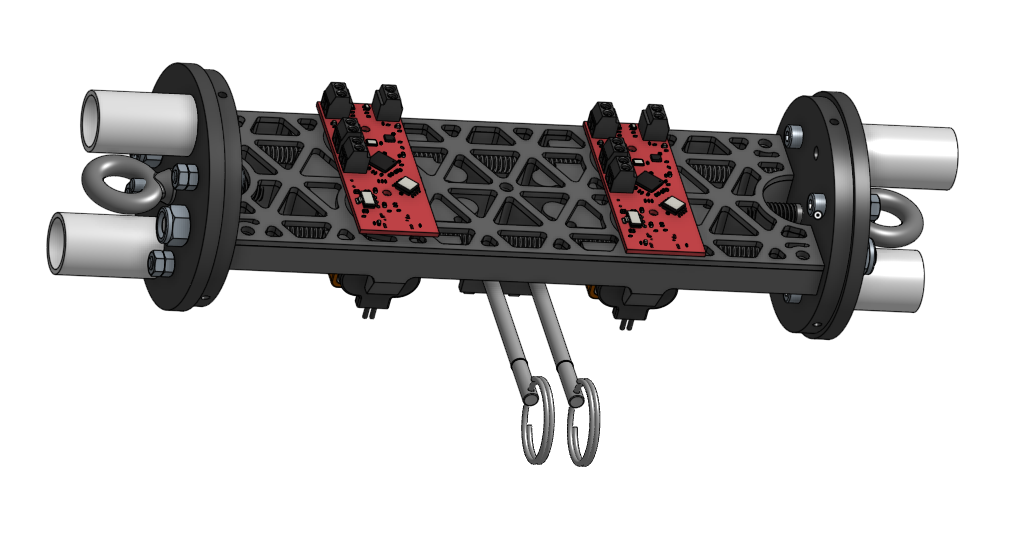
\includegraphics[width=1\linewidth]{Documentation/ARES/Use_Cases/Pics/COMET_CAD.png}
    \caption{CAD model of the COMET dual-deployment system.}
    \label{fig:COMET_CAD}
\end{figure}